% \usepackage{tikz}
% The following commands are not supported in PSTricks at present
% We define them conditionally, so when they are implemented,
% this pgf file will use them.
\ifx\du\undefined
  \newlength{\du}
\fi
\setlength{\du}{15\unitlength}
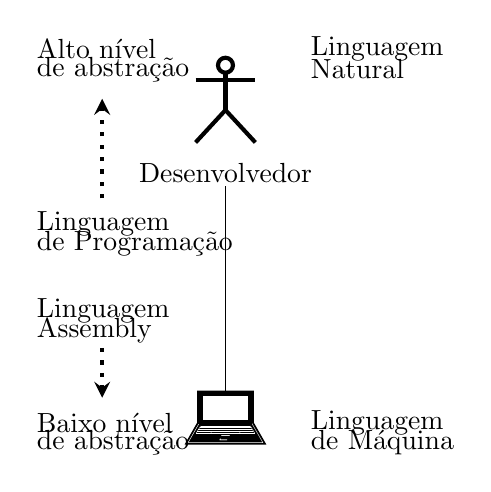
\begin{tikzpicture}
\pgftransformxscale{0.600000}
\pgftransformyscale{-0.600000}
\definecolor{dialineblack}{rgb}{0.0, 0.0, 0.0}
\definecolor{dialinewhite}{rgb}{1.0, 1.0, 1.0}
\definecolor{dialinegray}{rgb}{0.501961, 0.501961, 0.501961}
\pgfsetstrokecolor{dialineblack}
\pgfsetfillcolor{dialinewhite}
\pgfsetlinewidth{0.100000\du}
\pgfsetdash{}{0pt}

%Desenha o bonequinho
\pgfpathellipse{\pgfpoint{7.950000\du}{2.650000\du}}{\pgfpoint{0.300000\du}{0\du}}{\pgfpoint{0\du}{0.300000\du}}
\pgfusepath{fill}
\pgfpathellipse{\pgfpoint{7.950000\du}{2.650000\du}}{\pgfpoint{0.300000\du}{0\du}}{\pgfpoint{0\du}{0.300000\du}}
\pgfusepath{stroke}
\draw (6.750000\du,3.250000\du)--(9.150000\du,3.250000\du);
\draw (7.950000\du,2.950000\du)--(7.950000\du,4.450000\du);
\draw (7.950000\du,4.450000\du)--(6.750000\du,5.750000\du);
\draw (7.950000\du,4.450000\du)--(9.150000\du,5.750000\du);
\node at (7.950000\du,6.990000\du){Desenvolvedor};

%Desenha o computador
\pgfsetfillcolor{dialineblack}
\fill (6.894444\du,15.800000\du)--(9.005556\du,15.800000\du)--(9.005556\du,17.022222\du)--(9.450000\du,17.800000\du)--(6.450000\du,17.800000\du)--(6.894444\du,17.022222\du)--cycle;
\pgfsetstrokecolor{dialineblack}
\draw (6.894444\du,15.800000\du)--(9.005556\du,15.800000\du)--(9.005556\du,17.022222\du)--(9.450000\du,17.800000\du)--(6.450000\du,17.800000\du)--(6.894444\du,17.022222\du)--cycle;
\pgfsetlinewidth{0.010000\du}
\pgfsetbuttcap
\pgfsetmiterjoin
\pgfsetdash{}{0pt}
\pgfsetstrokecolor{dialinewhite}
\draw (6.894444\du,15.800000\du)--(9.005556\du,15.800000\du)--(9.005556\du,17.022222\du)--(9.450000\du,17.800000\du)--(6.450000\du,17.800000\du)--(6.894444\du,17.022222\du)--cycle;
\pgfsetbuttcap
\pgfsetmiterjoin
\pgfsetdash{}{0pt}
\definecolor{dialinecolor}{rgb}{0.501961, 0.501961, 0.501961}
\pgfsetstrokecolor{dialinecolor}
\draw (6.894444\du,17.022222\du)--(9.005556\du,17.022222\du);
\pgfsetlinewidth{0.100000\du}
\pgfsetbuttcap
\pgfsetmiterjoin
\pgfsetdash{}{0pt}
\definecolor{dialinecolor}{rgb}{1.000000, 1.000000, 1.000000}
\pgfsetfillcolor{dialinecolor}
\fill (6.950000\du,15.855556\du)--(8.950000\du,15.855556\du)--(8.950000\du,16.966667\du)--(6.950000\du,16.966667\du)--cycle;
\definecolor{dialinecolor}{rgb}{0.000000, 0.000000, 0.000000}
\pgfsetstrokecolor{dialinecolor}
\draw (6.950000\du,15.855556\du)--(8.950000\du,15.855556\du)--(8.950000\du,16.966667\du)--(6.950000\du,16.966667\du)--cycle;
\pgfsetlinewidth{0.010000\du}
\pgfsetbuttcap
\pgfsetmiterjoin
\pgfsetdash{}{0pt}
\definecolor{dialinecolor}{rgb}{0.000000, 0.000000, 0.000000}
\pgfsetstrokecolor{dialinecolor}
\draw (6.950000\du,15.855556\du)--(8.950000\du,15.855556\du)--(8.950000\du,16.966667\du)--(6.950000\du,16.966667\du)--cycle;
\pgfsetbuttcap
\pgfsetmiterjoin
\pgfsetdash{}{0pt}
\definecolor{dialinecolor}{rgb}{1.000000, 1.000000, 1.000000}
\pgfsetstrokecolor{dialinecolor}
\draw (6.866667\du,17.272222\du)--(9.033333\du,17.272222\du);
\pgfsetbuttcap
\pgfsetmiterjoin
\pgfsetdash{}{0pt}
\definecolor{dialinecolor}{rgb}{1.000000, 1.000000, 1.000000}
\pgfsetstrokecolor{dialinecolor}
\draw (6.825000\du,17.341667\du)--(9.075000\du,17.341667\du);
\pgfsetbuttcap
\pgfsetmiterjoin
\pgfsetdash{}{0pt}
\definecolor{dialinecolor}{rgb}{1.000000, 1.000000, 1.000000}
\pgfsetstrokecolor{dialinecolor}
\draw (6.908333\du,17.202778\du)--(8.991667\du,17.202778\du);
\pgfsetbuttcap
\pgfsetmiterjoin
\pgfsetdash{}{0pt}
\definecolor{dialinecolor}{rgb}{1.000000, 1.000000, 1.000000}
\pgfsetstrokecolor{dialinecolor}
\draw (6.783333\du,17.411111\du)--(6.950000\du,17.133333\du);
\pgfsetbuttcap
\pgfsetmiterjoin
\pgfsetdash{}{0pt}
\definecolor{dialinecolor}{rgb}{1.000000, 1.000000, 1.000000}
\pgfsetstrokecolor{dialinecolor}
\draw (9.116667\du,17.411111\du)--(8.950000\du,17.133333\du);
\pgfsetbuttcap
\pgfsetmiterjoin
\pgfsetdash{}{0pt}
\definecolor{dialinecolor}{rgb}{1.000000, 1.000000, 1.000000}
\pgfsetstrokecolor{dialinecolor}
\draw (6.783333\du,17.411111\du)--(9.116667\du,17.411111\du);
\pgfsetbuttcap
\pgfsetmiterjoin
\pgfsetdash{}{0pt}
\definecolor{dialinecolor}{rgb}{1.000000, 1.000000, 1.000000}
\pgfsetstrokecolor{dialinecolor}
\draw (6.950000\du,17.133333\du)--(8.950000\du,17.133333\du);
\pgfsetbuttcap
\pgfsetmiterjoin
\pgfsetdash{}{0pt}
\definecolor{dialinecolor}{rgb}{1.000000, 1.000000, 1.000000}
\pgfsetstrokecolor{dialinecolor}
\draw (7.366667\du,17.411111\du)--(7.387500\du,17.341667\du);
\pgfsetbuttcap
\pgfsetmiterjoin
\pgfsetdash{}{0pt}
\definecolor{dialinecolor}{rgb}{1.000000, 1.000000, 1.000000}
\pgfsetstrokecolor{dialinecolor}
\draw (8.512078\du,17.341671\du)--(8.512500\du,17.341667\du);
\pgfsetbuttcap
\pgfsetmiterjoin
\pgfsetdash{}{0pt}
\definecolor{dialinecolor}{rgb}{1.000000, 1.000000, 1.000000}
\pgfsetstrokecolor{dialinecolor}
\draw (8.533333\du,17.411111\du)--(8.512078\du,17.341671\du);
\pgfsetbuttcap
\pgfsetmiterjoin
\pgfsetdash{{1.000000\du}{1.000000\du}}{0\du}
\pgfsetdash{{0.200000\du}{0.200000\du}}{0\du}
\definecolor{dialinecolor}{rgb}{1.000000, 1.000000, 1.000000}
\pgfsetstrokecolor{dialinecolor}
\draw (7.783333\du,17.522222\du)--(8.116667\du,17.522222\du)--(8.172222\du,17.688889\du)--(7.727778\du,17.688889\du)--cycle;
% Mouse pad
\draw (7.783333\du,17.522222\du)--(8.116667\du,17.522222\du)--(8.172222\du,17.688889\du)--(7.727778\du,17.688889\du)--cycle;
\pgfsetbuttcap
{
\pgfsetdash{}{0pt}
\pgfsetfillcolor{dialineblack}
\pgfsetstrokecolor{dialineblack}
\draw (7.950000\du,7.50000\du)--(7.950000\du,15.800000\du);
}
\node[anchor=west] at (11.0    \du,2.0    \du){Linguagem};
\node[anchor=west] at (11.0    \du,2.800000\du){Natural};
\node[anchor=west] at (11.0    \du,17.0    \du){Linguagem};
\node[anchor=west] at (11.0    \du,17.800000\du){de Máquina};
\node[anchor=west] at (0.0    \du,2.0    \du){Alto nível};
\node[anchor=west] at (0.0    \du,2.800000\du){de abstração};
\node[anchor=west] at (0.0    \du,17.0    \du){Baixo nível};
\node[anchor=west] at (0.0    \du,17.800000\du){de abstração};
\node[anchor=west] at (0.0    \du,12.5    \du){Linguagem};
\node[anchor=west] at (0.0    \du,13.300000\du){Assembly};
\node[anchor=west] at (0.0    \du,9.0    \du){Linguagem};
\node[anchor=west] at (0.0    \du,9.800000\du){de Programação};
\pgfsetbuttcap
{
\pgfsetlinewidth{0.100000\du}
\pgfsetdash{{\pgflinewidth}{0.200000\du}}{0cm}
\pgfsetdash{{\pgflinewidth}{0.200000\du}}{0cm}
\pgfsetarrowsend{stealth}
\draw (3.0    \du,8.0    \du)--(3.0    \du,4.0    \du);
\draw (3.0    \du,14.0    \du)--(3.0    \du,16.0    \du);
}
\end{tikzpicture}
